%! Author = florian
%! Date = 25.05.23


\section{Eco-Friendly Consensus Mechanisms}\label{sec:eco-friendly-consensus-mechanisms}
This section will describe and compare alternative consensus mechanisms.
Around 60\% of the current consensus mechanisms used in blockchains is the POW(proof of work) consensus mechanism.
As already described in section\ \ref{sec:introduction}, the POW consensus mechanisms requires a miner to solve complex mathematical puzzles in order to create block on the blockchain.
This requires much energy and is therefore bad for the environment.\cite{overview-of-sustainablity-blockchains,moralis-pow-enery-consumption}

By moving to an alternative proof algorithm blockchains could reduce their energy consumption.
This section will describe these alternative consensus mechanisms.\cite{4-ways-to-counter-blockchains-energy-consumption}

\subsection{Proof of Stake}\label{subsec:proof-of-stake}
Proof of stake is the second most used consensus algorithm, next to proof of work.
Unlike proof of work, the proof of stake consensus algorithm does not need miners to create blocks for the blockchain.
Instead, participants, who want to create blocks, have to place a certain amount of the networks tokens as a stake.
These participants are known as validators.
The coins in a stake are locked and cannot be used for transactions.
If a validator wants to access the tokens in their stake, they have to stop being a validator in order to do so.
The amount of blocks they can create is limited by the size of the placed stake.
The creator of a blocks gets the transaction fees associated with the transactions in the block, but no mining reward.\cite{bitpanda-pos}

Another aspect of proof of stake is the penalty mechanism.
If a participant acts malicious or is, for example, offline they can get their stake slashed.
This means that the tokens that were staked are removed from the participants account.\cite{bitpanda-pos}

The nature of proof of stake is therefore a deterministic algorithm, since the creator of the block is selected by the size their stake.
This can lead to unwanted centralization, since a participant with many tokens has an advantage over participants with only a small amount of tokens.
To prevent the centralization of the network, there are other selection methods, such as:

\begin{itemize}
    \item\textbf{Stationary Time}: Validators are selected based on the amount of time their cryptocurrency has been locked up in the network.\cite{bitpanda-pos}
    \item\textbf{Coin Age}: Validators are selected based on the product of their stake and the amount of time the tokens have been held in the network.\cite{bitflyer-glossary}
    \item\textbf{Randomized Block Selection}: Validators are selected based on a pseudorandom function that combines their stake with other factors such as the hash of the previous block.\cite{cryptonews-pos}
\end{itemize}

\subsubsection{Pros and Cons of Proof of Stake}
As already mentioned proof of stake is more energy efficient, since nothing is actually calculated.
It also provides better throughput than proof of work and a lower entry barrier, because no special hardware is required to mine blocks.
One interesting aspect of proof of stake is, that it reduces centralization against mining farms, since more nodes can participate.
In that sense it reduces centralization.\cite{bitpanda-pos}

On the other hand proof of stake enables centralization, since validators with a higher stake have an advantage over participants with a lesser stake.
Proof of stake is also not as proven as proof of work.
If it is a viable alternative solution has to be shown.\cite{insider-pos-vs-pow}

One problem of proof of stake the nothing at stake problem.
If creating blocks, does not actually require doing anything, like in proof of work, participants could just create multiple parallel chains.
So stakers just create multiple parallel blocks in order to get the transaction fees.
The solution to this problem is penalizing participants who create multiple parallel blocks.


\subsection{Proof of Capacity}\label{subsec:proof-of-capacity}
Proof of capacity is a consensus mechanism, that does not use CPUs or GPUs to create blocks, but empty storage space.
Miners, or also called farmers in this case, use HDDs and SSDs to farm blocks.
The empty storage space is split into plots.
Each plot is a file on the storage device.
A plot is filled with precalculated proof of work functions.
If a new block has to be farmed, farmers simple scan their plots for the correct plot and can then farm the plot.

The greater the amount of storage space allocated by a node operator on their hard drive, the increased likelihood of finding a matching hash value from a predetermined list.
This, in turn, enhances their chances of winning the mining reward.
This requires large amount of free space on a hard-drive, but does not need much energy to create new blocks.\cite{chia-whitepaper,geeksforgeeks-poc}

There are a few other consensus mechanisms that are similar to proof of capacity.
Such as:
\begin{itemize}
    \item\textbf{Proof of Space}: The prover(farmer) sends a piece of data to a verifier, that proves that the farmer has reserved a certain amount of space on their storage device.
    It is similar to proof of stake, that is described in subsection\ \ref{subsec:proof-of-stake}, but it does use storage space instead of tokens.
    \item\textbf{Conditional Proof of Capacity} is a combination of proof of work, proof of stake, described in subsection\ \ref{subsec:proof-of-stake}, and proof of capacity.
    Miners can get a higher income by pledging additional tokens, similar to proof of stake.
\end{itemize}

\subsubsection{Pros and Cons of Proof of Capacity}
As all other consensus mechanisms mentioned in this section, proof of capacity is more eco-friendly than proof of work.
It does have the additional advantage, that it can be mined by anyone who has free storage space.
This is especially useful, if the farmer has free storage space for future use, but does not need it at the moment.
There is also no need for equipment upgrades, since old storage devices are still capable of storing data effectively.
After the farmer is done with farming, they can wipe the storage device and use it for other storage needs.

There are still a few limitations.
Storage devices have a limited capacity, so farmers might need to buy more storage devices to farm more efficiently.
There is still a centralization risk, if a limited number of miners control the majority of storage space.
Last, if a storage device fails, it is possible to loss stored data and therefore mining rewards.\cite{geeksforgeeks-poc}


\subsection{Proof of Space and Time}\label{subsec:proof-of-space-and-time}
Another alternative consensus mechanism is proof of space and time(PoST).
It requires participants to use storage space to validate transactions.
It is supposed to be more energy efficient than proof of work and proof of stake.

In more details, proof of space and time consists of two different consensus mechanisms, that are combined.
First, proof of space, this consensus mechanism reserves hard-drive space for mining blocks.
This approach is also described in subsection\ \ref{subsec:proof-of-capacity}.
Since proof of space does take little to no time to look up, a second consensus mechanism, called proof of time, is used.
Proof of time requires a small delay between blocks using a verifiable delay function or VDF\@.
The VDF takes a certain time to compute, but is fast to verify, similar to proof of work.
Unlike proof of work it requires sequential computation, so there is no benefit when using parallel GPUs or CPUs.
The workload is adjusted over time so the same amount of blocks are created over a timespan.
This delay is to stop miners from getting additional rewards when mining with large amounts of storage space.
It is still possible for participants to run multiple nodes.\cite{supraoracles-post,chia-whitepaper}

\subsubsection{Pros and Cons of Proof of Space and Time}
As already mentioned PoST is more energy efficient as it uses unused storage space rather than computation.
The hardware requirements to run a validator node is also lower, as it only requires free storage space.

One major disadvantage of PoSt its increased wear on HDDs and SSDs.
It can reduce the shelf life of a hard drive to only 40 days rather than the usual shelf life of a decade.
This also means, while PoST itself requires less energy, it may not be an eco-friendly solution, since validators will have to buy new hard drives more frequently and produce more waste.
Compared to the lifespan of a gpu that is used to mine cryptocurrencies, which is about three to five years, this is way less.
So while being more energy efficient, PoST is definitely not better for the environment.\cite{euronews-chia, devicetest-gpu-lifespan, supraoracles-post}

\subsection{Proof of Authority}\label{subsec:proof-of-authority}
The proof of authority consensus mechanism is very different to the other consensus algorithms already described in this section.
It is suitable for private blockchains.
In proof of authority not everybody can be a validator.
The validators are preselected based on their reputation, instead of using a stake or time and space.
To become a validator, the candidates identity has to be checked, and the candidate has to be willing to stake money and/or their reputation.
Usually, there should be a rigorous selection process to filter out questionable candidates.\cite{coindesk-poa}

\subsubsection{Pros and Cons of Proof of Authority}
There are multiple pros and cons on proof of authority.
An advantage of a blockchain based on proof of authority is that it can execute more transactions per second by not having to calculate a proof of work everytime a validator builds a block.
Blockchains using proof of authority are also better secured against 51\% attacks, since the validators are all highly vetted.
Validators also do not need special hardware to build blocks compared to proof of work or proof of space and time as mentioned in\ \ref{subsec:proof-of-space-and-time}.

A disadvantage would be the centralization of the blockchain, by having to check and identify each potential validator not every participant in the blockchain can become one.
Therefore, the blockchain loses the aspect of being decentralized as being show in figure\ \ref{fig:centralization-of-proof-of-authority}.
One key aspect of blockchains is their immutability.
This makes blockchains resilient to censorship and the blockchain is available to everyone.
By centralizing the validators the blockchain loses these abilities.
It is easier to block a specific participant  or manipulate the blockchain if the validators wish to do so.

Since the validator nodes are publicly known they are vulnerable to manipulation themselves.
An outside actor could try to influence validators to act in a dishonest or destructive way.\cite{insidecrypto-poa,coindesk-poa}

\begin{figure}[h]
    \centering
    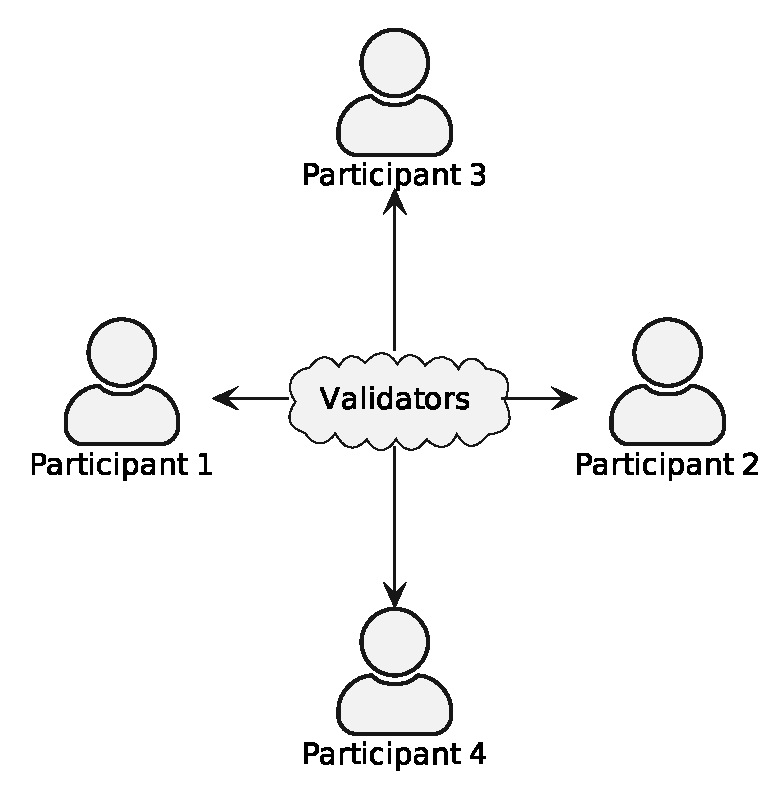
\includegraphics[scale=0.5]{img/proof-of-authority-0}
    \caption{Centralization of Proof of Authority}
    \label{fig:centralization-of-proof-of-authority}
\end{figure}

